%% eyeq_conference6.tex — IEEE CONFERENCE paper, 6-page limit
%%
%% EYEQ: A Hybrid Quantum--Classical Eye-Gaze Typing System on Commodity
%% Webcams
%%
%% Built on IEEEtran.cls v1.8b with the [conference] option. The journal
%% template's \markboth running headers and IEEEbiography blocks are
%% deliberately omitted: conference papers carry neither.
%%
%% Compile: pdflatex eyeq_conference6  (x2; the bibliography is inlined,
%% so bibtex is not required)

\documentclass[conference]{IEEEtran}

\usepackage{cite}
\usepackage{amsmath}
\usepackage{amssymb}
\usepackage{graphicx}
\usepackage{booktabs}
\usepackage{array}
\usepackage{stfloats}

\newtheorem{proposition}{Proposition}
\interdisplaylinepenalty=2500
\hyphenation{nor-mal-isa-tion cal-i-bra-tion land-mark}

\begin{document}

\title{EYEQ: A Hybrid Quantum--Classical Eye-Gaze\\
Typing System on Commodity Webcams}

\newcommand{\authname}[1]{{\normalfont\sublargesize #1}}
\newcommand{\authaff}[1]{{\normalfont\normalsize #1}}
\author{%
\renewcommand{\arraystretch}{0.9}%
\begin{tabular}[t]{@{}c@{\hspace{2.6em}}c@{}}
\begin{tabular}[t]{@{}c@{}}
\authname{Devash Sivakumar}\\
\authaff{Dept. of Computer Science and Engineering}\\
\authaff{Vels Institute of Science, Technology}\\
\authaff{and Advanced Studies}\\
\authaff{Chennai, India}\\
\authaff{23619110@vistas.ac.in}
\end{tabular}
&
\begin{tabular}[t]{@{}c@{}}
\authname{R. Anandan}\\
\authaff{Dept. of Computer Science and Engineering}\\
\authaff{Vels Institute of Science, Technology}\\
\authaff{and Advanced Studies}\\
\authaff{Chennai, India}\\
\authaff{anandan.se@vistas.ac.in}
\end{tabular}
\\ \noalign{\vskip 11.6pt}
\begin{tabular}[t]{@{}c@{}}
\authname{V. Maruthi}\\
\authaff{Dept. of Computer Science and Engineering}\\
\authaff{National Institute of Technology}\\
\authaff{Tiruchirappalli}\\
\authaff{Tiruchirappalli, India}\\
\authaff{maruthiphd.83@gmail.com}
\end{tabular}
&
\\
\end{tabular}}

\maketitle

\begin{abstract}
Eye typing on a commodity webcam faces two problems in series, and they are not
the same kind of problem: estimating a screen coordinate from a low-resolution
face, and committing a character from a noisy coordinate and a language
context. We address both. For the decision problem we introduce a
\emph{quantum conditional selection rule}: candidate keys occupy a five-qubit
register with amplitudes carrying the gaze likelihood, a language-conditioned
diagonal unitary attaches both magnitude and phase, a consistency oracle admits
only hypotheses that re-encode to what was gazed, and the Born rule commits. We
prove it contains the deployed log-linear fusion exactly at zero phase and that
its interference cross-terms are unreachable classically. Measured on identical
noise at matched prompt rate it is worth a median $-0.03$ percentage points, and
we give the mechanism: coherence is anti-correlated with correctness. For the
estimation problem we replace eyelid-relative normalisation of the iris offset
with a canthus-relative one, cutting held-out error from $5.55^\circ$ to
$3.76^\circ$ across eleven sessions from nine participants, improving every
participant, and roll-invariant by construction.
\end{abstract}

\begin{IEEEkeywords}
Quantum conditional selection rule; interference-based fusion; amplitude
amplification; eye-gaze typing; webcam gaze estimation; dwell selection;
assistive text entry; facial landmarks; calibration.
\end{IEEEkeywords}

% ---------------------------------------------------------------------------
\begin{figure}[!tb]
\centering
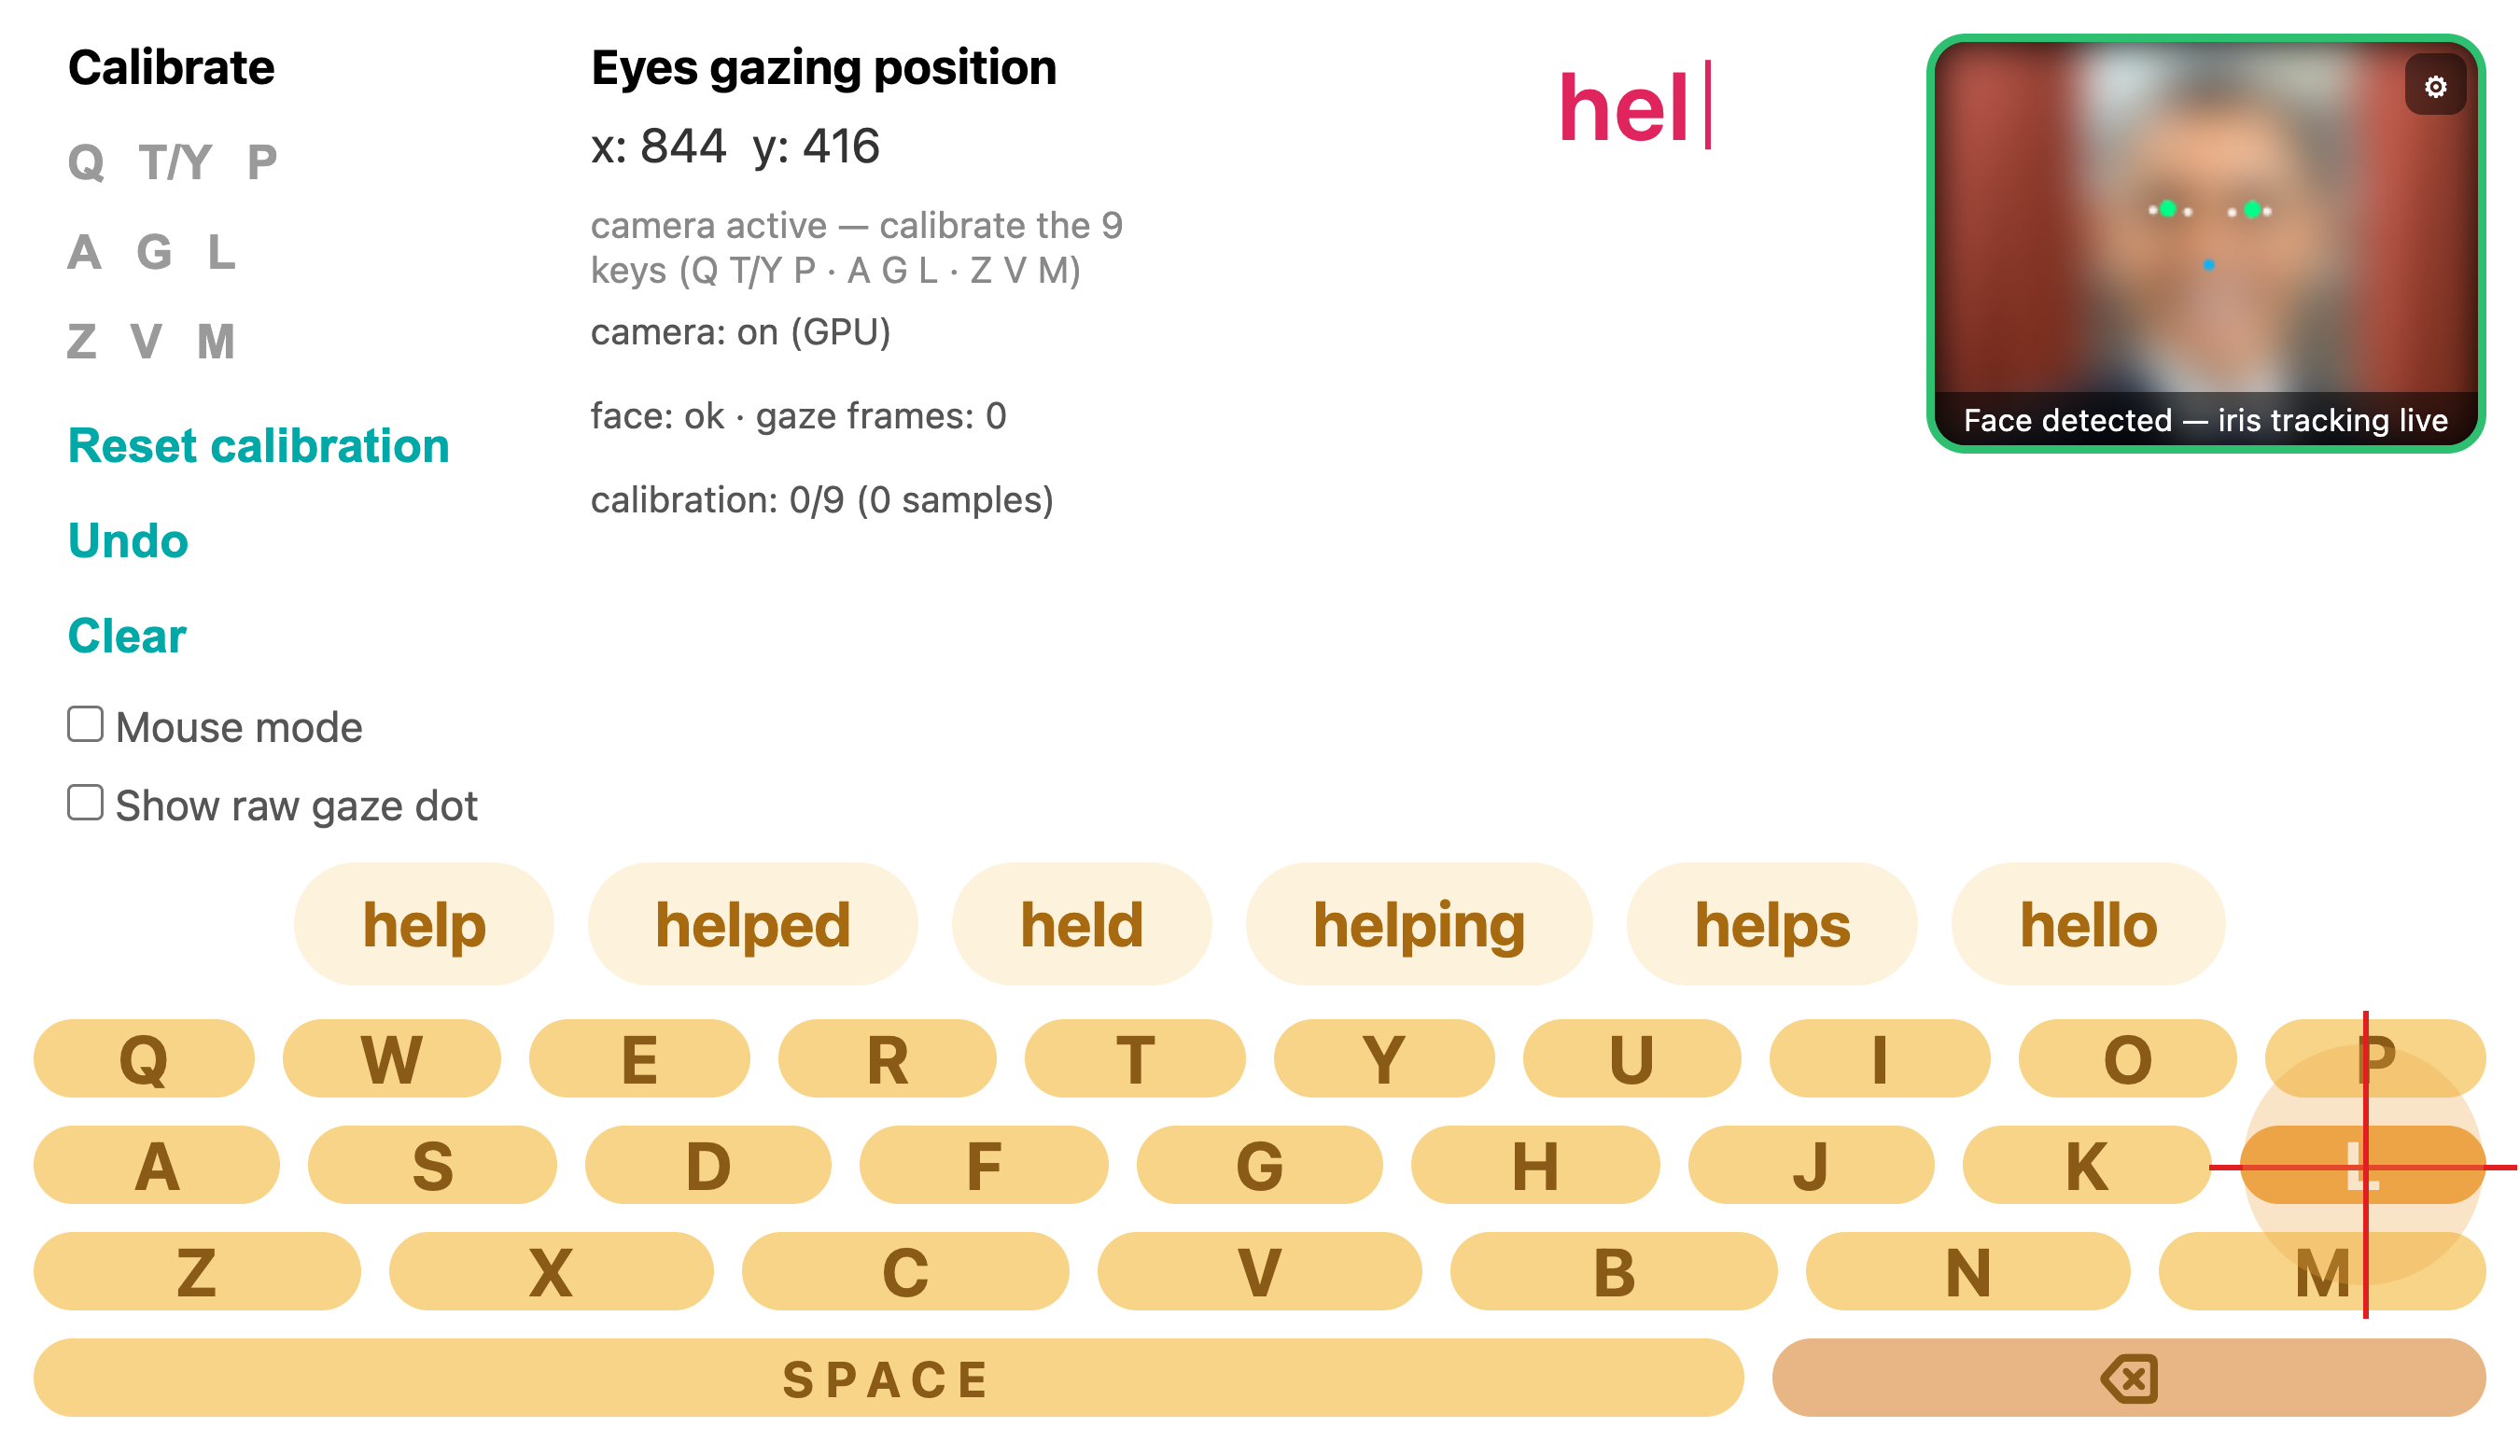
\includegraphics[width=\linewidth]{figs/fig_ui}
\caption{The deployed interface, captured live. In the preview panel the green
markers are the iris centres and the white markers beside them are the medial
and lateral canthi --- the landmarks \eqref{eq:canthus} is built on. The user
has gaze-typed \texttt{hel}; the crosshair rests on \textsf{L}, which is
filling its dwell, and the language model offers six completions. The camera
image is blurred for privacy; the tracking overlay is a separate canvas and is
unaffected.}
\label{fig:ui}
\end{figure}
% ---------------------------------------------------------------------------

\section{Introduction}

\IEEEPARstart{E}{ye} typing gives people with severe motor impairment a writing
channel that needs no limb movement. Infrared trackers reach $0.25$--$0.5^\circ$
of gaze error but cost more than the computers they attach to, so a large
literature pursues the same capability with a consumer webcam alone.
Fig.~\ref{fig:ui} shows the system this paper reports.

That literature reports \emph{classifiers}: the fraction of frames assigned to
the correct region, over two to nine regions, with figures of $85$--$93\,\%$
common. That is a fair measure of a fair design, since such systems select by
blinking or scanning and need only a coarse direction, but it is not comparable
to continuous angular error and cannot tell a reader whether a user could point
at a key. We take the harder formulation throughout --- a continuous coordinate,
held-out targets, degrees of visual angle --- and working in that regime exposed
a defect in a step the literature treats as settled.

The decision problem received the more ambitious treatment and returned less.
Gaze keyboards multiply a gaze posterior by a language prior, a product of
\emph{marginals}; a marginal has already discarded whether a letter's support
came from one confident word or fifty diffuse ones. Our rule keeps the
hypotheses distinct, places them in superposition with gaze-derived amplitudes,
and attaches a \emph{phase} to each so that context-coherent hypotheses
interfere. We prove no classical mixture can express that, measure it, and find
it worth nothing --- for a reason sharp enough to be the more durable
contribution.

\subsection{Contributions}

\begin{enumerate}
\item A quantum conditional selection rule for gaze--language fusion, with a
containment proposition showing it recovers the deployed log-linear fusion
exactly at zero phase and an expressiveness proposition showing its
cross-terms are unreachable classically.
\item A measured null with a diagnosed mechanism. Interference is worth a
median $-0.03$ percentage points at matched prompt rate because coherence is
\emph{anti}-correlated with correctness, and no retuning fixes a sign.
\item Canthus-relative normalisation, which cuts held-out error by $32.3\,\%$
across nine participants, subsumes explicit head pose, is roll-invariant by
construction to $\sim$$10^{-15}$, and explains an asymmetry reported but
undiagnosed in prior work ($93\,\%$ horizontal against $76\,\%$ vertical).
\end{enumerate}

\section{Related Work and Positioning}

Table~\ref{tab:survey} groups representative webcam gaze keyboards by how the
iris is localised, because that choice determines what the rest of the system
can do. Threshold-and-projection methods~\cite{ref08} are inexpensive but need a
per-illumination threshold. Circle fitting~\cite{ref09} is the only surveyed
work targeting dedicated hardware. The largest
group~\cite{ref02,ref03,ref05,ref07} uses the 68-point \emph{dlib} predictor and
derives an eye aspect ratio; that model contains \emph{no iris landmarks at
all}, which is why all four select keys by blinking or scanning rather than by
pointing. Only~\cite{ref04} and~\cite{ref06} adopt the dedicated iris ring of
MediaPipe~\cite{ref10}, the prerequisite for continuous regression. Enlarging targets and
recovering the word with a language model is the established trade in text
entry~\cite{ref17}; our addition is the constraint direction, since the oracle
of Section~\ref{sec:rule} admits only hypotheses that re-encode to exactly the
gazed sequence.

Two facts in Table~\ref{tab:survey} motivate this work. First, \textbf{no
surveyed work reports gaze error in degrees}, so our results cannot be ranked
against them and we do not attempt it. Second, \textbf{head pose is almost
entirely absent}: one work models it implicitly~\cite{ref01}, one
\emph{prohibits} head movement and reports the discomfort as a
limitation~\cite{ref02}, and one notes that head shaking causes error without
addressing it~\cite{ref09b}. Section~\ref{sec:results} explains why that
omission has cost less than expected.

% ---------------------------------------------------------------------------
\begin{table*}[!tb]
\renewcommand{\arraystretch}{1.2}
\caption{Representative Webcam Gaze-Keyboard Systems. The Rightmost Column is
the Point of the Table: Reported Figures Measure Region Classification, Not
Continuous Gaze Error, and Are Therefore Not Comparable With This Work.}
\label{tab:survey}
\centering
\footnotesize
\begin{tabular}{@{}p{2.6cm}p{5.2cm}p{4.0cm}p{4.2cm}@{}}
\toprule
\textbf{Work} & \textbf{Iris localisation} & \textbf{Head pose} &
\textbf{Reported} \\
\midrule
Waideman \emph{et al.}~\cite{ref01} & 4-stream CNN (face, eyes, head) & \textbf{Yes}, 4th channel & 93\,\% L/R, \textbf{76\,\% U/D} \\
Islam \emph{et al.}~\cite{ref02} & dlib 68-pt, midpoint & Movement prohibited & CPM/WPM only \\
Rafid \emph{et al.}~\cite{ref04} & \textbf{MediaPipe iris} & No & 14.53 CPM \\
Kathpal \emph{et al.}~\cite{ref07} & Horizontal/vertical gaze ratio & No & 91\,\% / 85\,\% (glasses) \\
Padilla \emph{et al.}~\cite{ref09} & Sobel + thinning + Circular Hough & No & FPGA $\equiv$ MATLAB \\
Li \emph{et al.}~\cite{ref09b} & SMI ETG 2w (commercial IR) & Noted, unsolved & --- \\
\midrule
\textbf{This work} & \textbf{MediaPipe iris, canthus-normalised} & \textbf{Implicit (canthus frame)} & $\mathbf{3.76^\circ}$ \textbf{continuous} \\
\bottomrule
\end{tabular}
\end{table*}
% ---------------------------------------------------------------------------

\section{Front End: Estimating the Coordinate}
\label{sec:frontend}

\subsection{The vertical-asymmetry observation}

The observation that motivates our method is already in the literature but is
not commented upon there. Waideman and Aquino Junior~\cite{ref01} report
directional accuracy split by axis, $93\,\%$ for left/right against $76\,\%$ for
up/down, and do not explain the gap. Consider how the vertical channel is
conventionally formed. With $\mathbf{p}$ the iris centre and $t$, $b$ the upper
and lower eyelid landmarks, the standard feature is
\begin{equation}
v = \frac{p_y - t_y}{b_y - t_y + \epsilon},
\label{eq:eyelid}
\end{equation}
the iris height as a fraction of the \emph{eyelid aperture}. That denominator is
not a fixed anatomical quantity: it contracts with every squint, every partial
blink, and with ambient brightness, so $v$ changes without the eye having moved.
The horizontal channel, normalised by the distance between the eye corners,
suffers no equivalent contamination. An eyelid-normalised vertical channel
should therefore be measurably worse than its horizontal counterpart, which is
what~\cite{ref01} reports. Our method follows directly: normalise against a
structure that does not move.

\subsection{Canthus-relative normalisation}

Let $\mathbf{i}$, $\mathbf{m}$ and $\mathbf{l}$ be the iris centre and the
medial and lateral canthi of one eye. We define the eye axis and its
perpendicular,
\begin{equation}
\mathbf{u} = \frac{\mathbf{m} - \mathbf{l}}{\lVert \mathbf{m} - \mathbf{l}\rVert},
\qquad
\mathbf{u}^{\perp} = \begin{bmatrix} -u_y \\ u_x \end{bmatrix},
\end{equation}
take the offset from the canthus midpoint as
$\mathbf{d} = \mathbf{i} - \tfrac{1}{2}(\mathbf{m} + \mathbf{l})$, and express
it in the eye's own frame, scaled by the inter-canthal distance
$w = \lVert \mathbf{m} - \mathbf{l}\rVert$:
\begin{equation}
c_{\parallel} = \frac{\mathbf{d}\cdot\mathbf{u}}{w},
\qquad
c_{\perp} = \frac{\mathbf{d}\cdot\mathbf{u}^{\perp}}{w}.
\label{eq:canthus}
\end{equation}

Two properties follow. The scale $w$ is a Euclidean distance rather than a
coordinate difference, so it does not collapse as the head turns. And because
$\mathbf{u}$ rotates with the head, \eqref{eq:canthus} is invariant to head roll
\emph{by construction} --- no roll angle is estimated, and none is needed.
Fig.~\ref{fig:geometry} contrasts the two normalisations.

\subsection{Feature vector and calibration}

The full vector concatenates the four conventional ratios, head translation and
scale proxies, a bias term, and the four canthus components, giving $d = 12$.
Screen coordinates come from ridge regression,
$\mathbf{W} = (\mathbf{F}^{\!\top}\mathbf{F} + \lambda\mathbf{I})^{-1}
\mathbf{F}^{\!\top}\mathbf{T}$, fitted to a nine-target per-user calibration of
five fixations each. Predictions pass through a One Euro
filter~\cite{ref11}, and dwell hysteresis retains the target until the estimate
leaves the key by a margin, which converts boundary jitter into a stable
selection.

% ---------------------------------------------------------------------------
\begin{figure}[!tb]
\centering
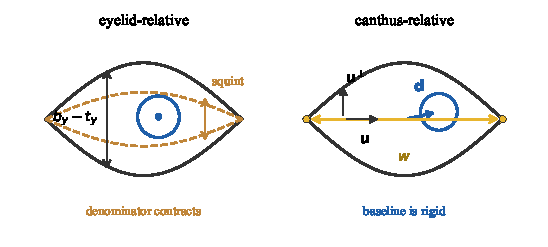
\includegraphics[width=\linewidth]{figs/fig_geometry}
\caption{Eyelid-relative against canthus-relative normalisation of the iris
offset. Only the latter is invariant to eyelid aperture and to head roll.}
\label{fig:geometry}
\end{figure}
% ---------------------------------------------------------------------------

\section{A Quantum Conditional Selection Rule}
\label{sec:rule}

\subsection{The rule}

At commit time the deployed system scores each candidate key $k$ as
\begin{equation}
\mathrm{score}(k) = P(k \mid \text{gaze}) \cdot
  \max\!\big(P(k \mid \text{prefix}),\, \varepsilon\big)^{\beta},
\label{eq:loglinear}
\end{equation}
with $\beta < 1$ damping the prior so the language model advises rather than
vetoes. The second factor is a marginal: the total frequency mass of every
vocabulary word continuing the prefix with $k$. Forming that sum destroys the
distinction between a letter backed by one dominant continuation and one backed
by a diffuse spray agreeing on nothing else.

Our rule keeps the hypotheses. Let $H$ be the vocabulary completions of the
current prefix, each with weight $w_h$ and proposing next letter $k_h$.
Candidates occupy a five-qubit register spanning $a$--$z$ and a word boundary,
prepared as $\lvert\psi\rangle = \sum_k \sqrt{P(k\mid\text{gaze})}\,\lvert
k\rangle$. Writing $v_h = w_h / P(k \mid \text{prefix})$ for the within-letter
weights, so $\sum_h v_h = 1$, a language-conditioned diagonal unitary gives
\begin{equation}
a(k) = \sqrt{P(k \mid \text{gaze})}\;
       P(k \mid \text{prefix})^{\beta/2}\;
       \underbrace{\textstyle\sum_{h:\,k_h = k} v_h\, e^{i\varphi_h}}_{c(k)},
\label{eq:rule}
\end{equation}
and the Born rule commits $\arg\max_k \lvert a(k)\rvert^{2}$. The factor $c(k)$
is the \emph{coherence} of letter $k$, a weighted mean phasor whose squared
modulus $\sum_{h}\sum_{h'} v_h v_{h'} \cos(\varphi_h - \varphi_{h'})$ carries
the interference in its off-diagonal terms. Since $\lvert c(k)\rvert \le 1$ with
equality exactly when the supporting hypotheses agree in phase, coherence
penalises letters reachable only through mutually incoherent continuations.
Phases come from each hypothesis's mean per-character log-frequency, rescaled to
$[0,1]$ over $H$ and multiplied by a scale $\sigma_\varphi\pi$.

\subsection{Containment and expressiveness}

\begin{proposition}[Containment]
\label{prop:contain}
At $\sigma_\varphi = 0$, \eqref{eq:rule} reduces to \eqref{eq:loglinear}.
\end{proposition}

\noindent\emph{Proof.} With all $\varphi_h = 0$, $c(k) = \sum_h v_h = 1$ for
every $k$, so $\lvert a(k)\rvert^{2} = P(k\mid\text{gaze})\,
P(k\mid\text{prefix})^{\beta}$, which is~\eqref{eq:loglinear} up to the shared
normalisation. $\square$

This is not a formality. A model class that cannot express the incumbent cannot
be said to have beaten it, so the comparison in Section~\ref{sec:results} is
meaningful only because the baseline lies strictly inside the family being
tested. We assert the identity numerically to $10^{-12}$ over randomised inputs
rather than relying on the derivation.

\begin{proposition}[Expressiveness]
\label{prop:express}
No classical mixture over the same hypotheses reproduces the cross-terms
of~\eqref{eq:rule}.
\end{proposition}

\noindent\emph{Proof sketch.} A mixture assigns letter $k$ probability
$\sum_h v_h^{2}$ after normalisation --- the diagonal alone. The off-diagonal
terms depend on phase differences, and a mixture has no phase. Since
$(\sum_h v_h)^{2} > \sum_h v_h^{2}$ whenever more than one hypothesis
contributes, the two disagree. $\square$

Concretely, two hypothesis sets with \emph{identical} marginals, and therefore
indistinguishable to~\eqref{eq:loglinear}, receive different posteriors
under~\eqref{eq:rule}, and the diffuse set is the one penalised.

\subsection{Oracle, amplification and cost}

The cluster decoder's correctness guarantee is a predicate: a hypothesis is
admissible only if re-encoding it reproduces exactly the cluster sequence
gazed. As an operator this is a projector $O_S$, and it is what prevents the
language model from ever proposing a word the gaze did not support. Given a
projector, amplitude amplification~\cite{ref13}, the generalisation of Grover
search~\cite{ref14} to a non-uniform start, rotates amplitude into the marked
subspace in $O(1/\sqrt{p_S})$ steps with
$m = \lfloor(\pi/4)/\arcsin\sqrt{p_S}\rfloor$ rounds. The intent is a shorter
dwell; Section~\ref{sec:results} reports what happens instead.

Twenty-seven candidates occupy a $32$-amplitude register, so the whole rule is a
handful of vector operations costing microseconds inside a $33$\,ms frame
budget. We claim no quantum speedup and simulate no hardware: the claim concerns
the rule's functional form, and the amplitude encoding is a product of
per-feature factors and therefore classically simulable by construction.

\section{Evaluation Protocol}
\label{sec:protocol}

Each session presents 21 targets, 13 for fitting and 8 held out at positions
spanning corner, edge and centre, with five fixations of 300\,ms retained per
target after discarding the first 150\,ms. Screen dimensions and viewing
distance are recorded, so the conversion to degrees is measured, not assumed.

All splits are \textbf{grouped by target}. The five fixations at one position
are one observation measured five times; splitting by sample leaves
near-identical siblings in the training set and selects a regulariser far too
small. Results are leave-one-target-out over all 21 positions, and the unit of
analysis is the participant, not the frame.

The selection rule is evaluated by end-to-end typing simulation over a
$16{,}839$-word vocabulary, the gaze likelihood being the exact Gaussian
integral over key rectangles at $\sigma \in \{30,40,50,60,75\}$\,px against a
$100\times110$\,px key. Three points carry the comparison. Both arms are driven
from one seeded generator, so any difference is the rule alone. Because a prompt
always yields the correct character, any rule reaches $100\,\%$ accuracy by
prompting constantly, so we sweep the threshold and compare \textbf{commit
accuracy at matched prompt rate}. And $\sigma_\varphi$ is tuned on a
$60$-sentence training split and reported on a disjoint one, because a gain that
does not survive the split is not a gain.

\section{Results}
\label{sec:results}

\subsection{The front end: canthus normalisation}

Canthus normalisation is the paper's largest effect.
Table~\ref{tab:ablation} puts held-out error at $5.552 \pm 0.488^\circ$ for the
deployed eyelid-relative features and $3.762 \pm 0.438^\circ$ with the canthus
components added, a reduction of $1.791^\circ$ or $32.3\,\%$. The comparison is
paired within participant over eleven sessions from nine participants:
$t(8) = 9.31$, $p = 1.4\times10^{-5}$, Wilcoxon $W = 0$, $p = 0.0039$,
$d_z = 3.10$, with a $95\,\%$ confidence interval on the reduction of
$[1.35, 2.23]^\circ$. \emph{Every one of the nine participants improved}, by
between $19.5\,\%$ and $44.6\,\%$; Fig.~\ref{fig:ablation} overlays all nine.

Three rows isolate the cause. An iris-ring radius cue yields $0.4\,\%$, well
within noise, so the gain is attributable to the canthi and not merely to having
more features. Head pose alone is worth $5.7\,\%$ --- the size of the effect the
canthus frame subsumes --- yet added \emph{on top of} that frame it yields
nothing detectable ($p = 0.439$), because the canthus frame is already
head-attached and an explicit pose stage re-derives information the
representation has removed. The same holds for radius ($p = 0.071$) and both
together ($p = 0.112$), while removing canthus normalisation costs
$40$--$47\,\%$ at $p < 0.001$. It is therefore the minimal sufficient addition,
not one useful feature among several.

Roll invariance holds numerically as well as analytically: rotating a synthetic
face through $0$--$40^\circ$, the canthus components drift by $4\times10^{-16}$
to $2\times10^{-15}$ while an image-axis formulation of the same offset drifts
by $0.069$. We report this as a property of the representation rather than a
measured gain, because the achieved roll across our sessions never exceeds
$6.5^\circ$ --- participants tilt far less than they are asked to.

% ---------------------------------------------------------------------------
\begin{figure}[!tb]
\centering
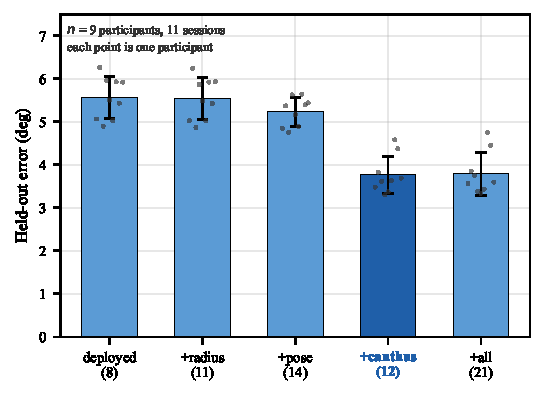
\includegraphics[width=\linewidth]{figs/fig_ablation}
\caption{Held-out error by feature set. Bars are the mean across the nine
participants and whiskers one standard deviation; each participant contributes
the mean of their own sessions, and all nine are overlaid as points so the
spread is visible rather than summarised. Every participant improves under
canthus normalisation, and adding iris radius or head pose on top of it changes
nothing detectable.}
\label{fig:ablation}
\end{figure}
% ---------------------------------------------------------------------------

% ---------------------------------------------------------------------------
\begin{table}[!tb]
\renewcommand{\arraystretch}{1.25}
\caption{Feature Ablation. Leave-One-Target-Out Over 21 Positions, Eleven
Sessions From Nine Participants. Lower is Better.}
\label{tab:ablation}
\centering
\footnotesize
\begin{tabular}{@{}lccc@{}}
\toprule
\textbf{Feature set} & \textbf{Dim} & \textbf{Error (deg)} &
\textbf{vs deployed} \\
\midrule
Deployed (eyelid-relative) & 8  & $5.552 \pm 0.488$ & baseline \\
\quad + iris-ring radius   & 11 & $5.529 \pm 0.488$ & $+0.4\,\%$ \\
\quad + head pose only     & 14 & $5.233 \pm 0.337$ & $+5.7\,\%$ \\
\textbf{\quad + canthus}   & \textbf{12} & $\mathbf{3.762 \pm 0.438}$ &
$\mathbf{+32.3\,\%}$ \\
\quad + canthus + pose     & 21 & $3.788 \pm 0.493$ & $+31.8\,\%$ \\
\quad + all of the above   & 24 & $3.663 \pm 0.474$ & $+34.0\,\%$ \\
\bottomrule
\multicolumn{4}{@{}p{7.6cm}@{}}{\footnotesize Mean $\pm$ standard deviation over
the nine participants, each contributing the mean of their sessions. Adding
radius, pose or both on top of the canthus frame changes nothing detectable
($p = 0.071$, $0.439$, $0.112$).}
\end{tabular}
\end{table}
% ---------------------------------------------------------------------------

\subsection{The selection rule at matched prompt rate}

The interference channel does not pay. Tuned on the training split, the best
phase scale was $\sigma_\varphi = 0.40$, worth $+0.03$ percentage points there.
On held-out sentences that advantage disappears: across twenty
$(\sigma, \text{prompt rate})$ cells, four of which Table~\ref{tab:selection}
shows, the median change is $-0.03$ percentage points, with zero significant
wins and zero losses.
The two posteriors do differ, just negligibly and without direction --- the mean
Kullback--Leibler divergence is $4.2\times10^{-4}$ nats per keystroke --- so the
null is not an artefact of a rule that fails to engage. Nor is it an artefact of
too small a scale: scales above $0.6$ produce substantial interference and
\emph{lose}, falling from $97.0\,\%$ to $95.3\,\%$ on the training split as
$\sigma_\varphi$ rises from $0$ to $1.0$.

Amplitude amplification does not shorten dwell either. Applied after the
conditioning unitary it is a no-op by construction: the conditioned state
already places $94$--$98\,\%$ of its amplitude on consistent letters, so the
optimal round count evaluates to zero and the operator never fires. The
quadratic speedup is real but addresses a bottleneck this system does not have,
because the admissible subspace is not rare. Forced to act on the raw gaze
register, mean dwell rises from $2.63$ to $2.80$ frames and commit accuracy
falls from $98.4\,\%$ to $96.4\,\%$ ($p = 0.48$, paired over the 249 keystrokes
both arms committed).

% ---------------------------------------------------------------------------
\begin{figure}[!tb]
\centering
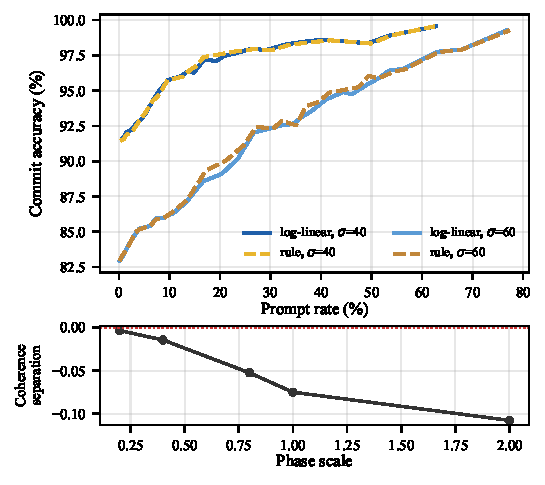
\includegraphics[width=\linewidth]{figs/fig_selection}
\caption{Top: the selection rule traces the same accuracy/prompt-rate frontier
as the fusion it generalises, at both noise levels. Bottom: the reason. The
coherence separation between correct and incorrect letters is negative at every
phase scale and falls monotonically, so the interference penalty lands on the
correct letter rather than on the wrong ones.}
\label{fig:selection}
\end{figure}
% ---------------------------------------------------------------------------

\subsection{Why interference fails: a sign, not a magnitude}

A null result is more useful with a mechanism attached, and this one is sharp.
For interference to help, the coherence penalty must fall more heavily on wrong
letters than on right ones. Fig.~\ref{fig:selection} measures it, and it is
negative at every phase scale, worsening monotonically from $-0.004$ at
$\sigma_\varphi = 0.2$ to $-0.108$ at $\sigma_\varphi = 2.0$. The upper panel
shows the consequence: the two frontiers lie on top of one another.

The cause is structural. The correct letter following an English prefix is
typically the one with the \emph{richest} vocabulary support: many genuine
continuations, therefore many hypotheses, therefore the widest spread of phases
and the lowest coherence. A wrong letter is typically backed by one obscure
completion and sits at coherence $1$. Any phase computed from hypothesis
likelihood thus penalises the letter with the strongest linguistic evidence. We
rejected two alternative explanations: raising the hypothesis budget from $4$ to
$4096$ moves mean coherence only from $0.982$ to $0.988$, and flattening the
within-letter weights to uniform changes it from $0.9883$ to $0.9879$. The
limitation is the phase \emph{source}. A language model offers no feature
orthogonal to the likelihood that already sets the magnitude, so the phase
channel carries no independent information for interference to exploit.

% ---------------------------------------------------------------------------
\begin{table}[!tb]
\renewcommand{\arraystretch}{1.25}
\caption{Selection Rule Against Deployed Log-Linear Fusion, Held-Out, at
Matched Prompt Rate. Each Cell Gives the Baseline Commit Accuracy and the
Rule's Change.}
\label{tab:selection}
\centering
\footnotesize
\begin{tabular}{@{}lccc@{}}
\toprule
$\sigma$ (px) & \textbf{2\,\% prompts} & \textbf{10\,\%} & \textbf{20\,\%} \\
\midrule
30 & 0.971\, $+$0.003 & 0.986\, $-$0.001 & 0.988\, $-$0.000 \\
40 & 0.921\, $-$0.002 & 0.958\, $-$0.000 & 0.973\, $+$0.003 \\
50 & 0.888\, $-$0.002 & 0.914\, $-$0.004 & 0.945\, $-$0.001 \\
60 & 0.841\, $-$0.000 & 0.862\, $+$0.001 & 0.891\, $+$0.008 \\
75 & 0.778\, $-$0.000 & 0.819\, $+$0.001 & 0.851\, $-$0.004 \\
\bottomrule
\multicolumn{4}{@{}p{7.6cm}@{}}{\footnotesize Median change over all twenty
$(\sigma, \text{prompt rate})$ cells $-0.0003$; significant wins \textbf{0},
losses \textbf{0}, by paired Wilcoxon over sentences.}
\end{tabular}
\end{table}
% ---------------------------------------------------------------------------


\section{Limitations}
\label{sec:limits}

Nine participants from one institution are not a sample of the population that
would use an assistive keyboard, so $[1.35, 2.23]^\circ$ describes this group
rather than eye geometry in general. Four participants contributed two sessions
and five contributed one, so between-session variance rests on four people.

The eyelid mechanism is supported but not demonstrated causally. The decisive
experiment holds the gaze target fixed while perturbing eyelid aperture, and the
prediction is specific: eyelid-relative features should degrade sharply and
canthus-relative features should not.

The selection-rule results come from simulation, with isotropic Gaussian noise
standing in for the anisotropic, correlated error a real tracker produces. The
null is specific to one vocabulary and one language --- our claim is that
likelihood-derived phase is mis-signed for English letter prediction, not that
interference-based fusion is useless --- and since coherence is the first
quantity a noisy device degrades, a null obtained in exact simulation is if
anything optimistic.

\textbf{Populations this system does not serve.} Two exclusions are boundaries
of applicability rather than shortfalls in accuracy, and we state them because
an assistive technology that overstates its reach does harm. The method assumes
a commanded fixation is held, so \emph{oculomotor instability} breaks it by
design: nystagmus leaves no stable fixation to average, strabismus means a
binocular iris average corresponds to no single gaze direction, and saccadic
intrusions defeat the dwell centroid. This is pointed, because motor-impaired
users are more likely to present with these conditions, and a scanning interface
remains the appropriate design there. \emph{Corrective eyewear} refracts the
apparent iris position, reflects under overhead light, and occludes the lateral
canthus at moderate yaw --- removing the very landmark \eqref{eq:canthus} is
built on. We did not record spectacle wearers, and the accuracy reported here
should not be expected to hold for them.

\section{Conclusion}

We set out to improve how a gaze keyboard decides, and improved how it estimates
instead. The quantum conditional selection rule is a strict generalisation of
log-linear fusion: it recovers the incumbent exactly at zero phase, and its
interference cross-terms are provably beyond any classical mixture of the same
hypotheses. Measured on identical noise at matched prompt rate it is worth a
median $-0.03$ percentage points, and amplitude amplification lengthens dwell
rather than shortening it.

The explanation is the more durable contribution. Interference fails here for a
reason no retuning addresses: the correct letter after an English prefix has the
richest vocabulary support, hence the most hypotheses, the widest phase spread
and the lowest coherence. Phase derived from hypothesis likelihood penalises
exactly the evidence it should reward. For interference to be useful, phase must
come from a source orthogonal to the magnitude, and a language model does not
provide one.

The accuracy came from the front end. Measuring a continuous coordinate in
degrees, rather than as region classification, exposed a defect in a step the
literature treats as settled: normalising the iris offset by the eyelid aperture
couples the vertical channel to a structure that moves independently of gaze.
Normalising against the canthi instead cuts held-out error by $32.3\,\%$ across
nine participants, improves every one of them, explains an axis asymmetry
reported but undiagnosed in prior work, and makes an explicit head-pose stage
unnecessary --- for four features and no additional runtime cost.

\section*{Acknowledgment}

The authors gratefully acknowledge the National Institute of Technology
Tiruchirappalli for providing access to its laboratory facilities, under which
this work was initiated and carried out to completion. The authors also thank
the Department of Computer Science and Engineering, Vels Institute of Science,
Technology and Advanced Studies, for its continued support.

% Balance the two columns on the last page: without this the references all
% land in the left column and the right one is empty. \IEEEtriggeratref{N}
% ends the column just before reference N. Retune N if the text length changes.
\IEEEtriggeratref{4}

\begin{thebibliography}{18}
\scriptsize

\bibitem{ref01}
B.~Waideman and P.~T. Aquino Junior, ``Augmentative and alternative
communication using eye tracking and word recommendation using language
models,'' \emph{IEEE Latin America Transactions}, vol.~23, no.~8,
pp.~637--645, Aug. 2025.

\bibitem{ref02}
M.~R. Islam, M.~S. Rahman, and A.~Sarkar, ``Computer vision based eye gaze
controlled virtual keyboard for people with quadriplegia,'' in \emph{Proc. Int.
Conf. Automation, Control and Mechatronics for Industry 4.0 (ACMI)}, Rajshahi,
Bangladesh, Jul. 2021, pp.~1--6.

\bibitem{ref03}
V.~Abhaya, A.~S. Bharadwaj, C.~C. Bagan, K.~Dhanraj, and G.~Shyamala,
``Eye-Move: An eye gaze typing application with OpenCV and Dlib library,'' in
\emph{Proc. Int. Conf. Automation, Computing and Renewable Systems (ICACRS)},
Dec. 2022, pp.~952--957.

\bibitem{ref04}
S.~T.~S. Rafid, A.~J. Ajwad, and A.~K.~M.~A.~M. Azad, ``Empowering quadriplegic
patients: A computer vision based approach for keyboard control using eye gaze
and blink,'' in \emph{Proc. 26th Int. Conf. Computer and Information Technology
(ICCIT)}, Cox's Bazar, Bangladesh, Dec. 2023, pp.~1--5.

\bibitem{ref05}
B.~G. Varshini, A.~Manimegalai, S.~D. Abirami, and S.~Kalaiselvi, ``Eye-gaze
controlled virtual keyboard using blink detection for accessible hands-free
communication,'' in \emph{Proc. Int. Conf. Computational, Communication and
Information Technology (ICCCIT)}, Feb. 2025, pp.~49--56.

\bibitem{ref06}
A.~SK, E.~D.~A, H.~B, and H.~M, ``Eye gaze tracking for virtual mouse control
using computer vision,'' in \emph{Proc. 4th Int. Conf. Artificial Intelligence
and Machine Learning Applications (AIMLA)}, Apr. 2026, pp.~1--6.

\bibitem{ref07}
K.~Kathpal, S.~Negi, and S.~Sharma, ``iChat: Interactive eyes for specially
challenged people using OpenCV Python,'' in \emph{Proc. 9th Int. Conf.
Reliability, Infocom Technologies and Optimization (ICRITO)}, Noida, India,
Sep. 2021, pp.~1--5.

\bibitem{ref08}
V.~I. Saraswati, R.~Sigit, and T.~Harsono, ``Eye gaze system to operate virtual
keyboard,'' in \emph{Proc. Int. Electronics Symp. (IES)}, Denpasar, Indonesia,
Sep. 2016, pp.~175--179.

\bibitem{ref09}
D.~A. Padilla, J.~A.~B. Adriano, J.~R. Balbin, I.~G. Matala, J.~J.~R. Nicolas,
and S.~R.~R. Villadelgado, ``Implementation of eye gaze tracking technique on
FPGA-based on-screen keyboard system using Verilog and MATLAB,'' in
\emph{Proc. IEEE Region 10 Conf. (TENCON)}, Penang, Malaysia, Nov. 2017,
pp.~2771--2776.

\bibitem{ref09b}
D.~Li, L.~Zhang, W.~Hu, H.~Li, and X.~Zhou, ``Dwell time adaptive three-way
text entry by gaze,'' in \emph{Proc. 31st Chinese Control and Decision Conf.
(CCDC)}, Nanjing, China, Jun. 2019, pp.~5295--5300.

\bibitem{ref10}
C.~Lugaresi \emph{et al.}, ``MediaPipe: A framework for building perception
pipelines,'' 2019, arXiv:1906.08172.

\bibitem{ref11}
G.~Casiez, N.~Roussel, and D.~Vogel, ``The one Euro filter: A simple
speed-based low-pass filter for noisy input in interactive systems,'' in
\emph{Proc. ACM CHI}, 2012, pp.~2527--2530.

\bibitem{ref13}
G.~Brassard, P.~H{\o}yer, M.~Mosca, and A.~Tapp, ``Quantum amplitude
amplification and estimation,'' in \emph{Quantum Computation and Information},
AMS Contemporary Mathematics, vol.~305, 2002, pp.~53--74.

\bibitem{ref14}
L.~K. Grover, ``A fast quantum mechanical algorithm for database search,'' in
\emph{Proc. 28th Annu. ACM Symp. Theory of Computing (STOC)}, 1996,
pp.~212--219.

\bibitem{ref17}
P.~O. Kristensson and S.~Zhai, ``SHARK$^2$: A large vocabulary shorthand
writing system for pen-based computers,'' in \emph{Proc. ACM UIST}, 2004,
pp.~43--52.

\end{thebibliography}

\end{document}
